\documentclass[10pt,a4paper]{article}
\usepackage[utf8]{inputenc}
\usepackage[russian]{babel}
\usepackage{amsmath}
\usepackage{amsfonts}
\usepackage{amssymb}
\usepackage{graphicx}
\usepackage{listings}
\lstset{
basicstyle=\small\ttfamily,
columns=flexible,
breaklines=true
}
\author{Дмитрий Баринов}
\title{Отчет по лабораторной работе№5 SSL}
\begin{document}
\maketitle
\newpage

\section{Цель работы}

Научиться развертывать SSL/TLS сервер.

\section{Ход работы}

\subsection{Лучшие практики по развертыванию SSL/TLS}

1. Использовать 2048-битные ключи.

2. Закрывайте приватные ключи.

3. Позабодьтесь о достаточном покрытии доменных имен.

4. Получайте сертификаты у надежных CA.

5. Используйте криптостойкие алгоритмы для подписей.

6. Настраивайте сервер для работы с несколькими сертификатами.

7. Используйте безопасные протоколы.

8. Используйте криптостойкие алгоритмы шифрования. Ключ не меннее 128 бит.

9. Используйте Forward Secrecy, позволяющую защищенный обмен, не зависящий от приватного ключа сервера.

10. Если нет необходимости, отключайте проверку защищенности соединения на стороне клиента.

11. Адаптируйте свою систему. Устанавливайте патчи к модулям защиты, когда они появляются.

12. Надо найти комромис между защищенностью системы и производительностью.

13. Шифруйте 100% вашего сайта.

14. ИСпользуйте защищенные куки.


\subsection{Изучить основные уязвимости и атаки на SSL последнего времени – POODLE, HeartBleed}

\paragraph{HeartBleed}
Уязвимости подвержаны следующие версии
OpenSSL 1.0.1 до 1.0.1f включительно.

Суть ошибки - неконтролируемое переполнение буфера, позволяющее несанкционированно читать память на сервере или на клиенте, в том числе для извлечения закрытого ключа сервера. Информация об уязвимости была опубликована в апреле 2014 года, ошибка существовала с конца 2011 года.


\paragraph{POODLE}
Суть уязвимости: злоумышленник может заставить обе стороны перейти на ssl 3.0, в котором используется потоковое шифрование RC4, которое, при больших объемах трафка, позволяет получить информацию, помогающее дешифрованию.


\subsection{Практическое задание: Выбрать со стартовой страницы SSL Server Test один домен из списка Recent Best и один домен из списка Recent Worst – изучить отчеты, интерпретировать результаты в разделе Summary}

\subsubsection{SSL Report: spsu.edu (168.28.176.243)}

\begin{figure}[h!]
\centering
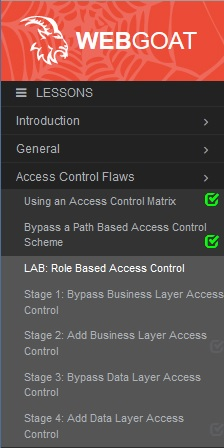
\includegraphics[scale=0.6]{1.jpg}
\caption{SSL Report: spsu.edu}
\end{figure}

Сервер защищен от DownGrade атаки. Но принимает уязвимое RC4 шифрование. Так же сервер не оддерживает Forward Secrecy.


\subsubsection{SSL Report: ica-corp.ica.com (72.167.40.106)}

\begin{figure}[h!]
\centering
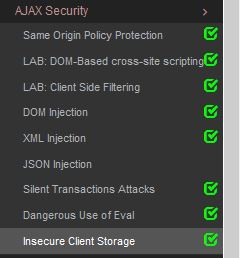
\includegraphics[scale=0.6]{2.jpg}
\caption{SSL Report: spsu.edu}
\end{figure}

У сервера нет доверенного сертификата. Не оддерживает Forward Secrecy. Но защищен от DownGrade атаки.

\subsection{Расшифровать все аббревиатуры шифров в разделе Configuration}

Каждая строка содержит информацию об используемых алгоритмах:
\begin{enumerate}
\item для обмена ключами
\item для шифрования сообщений
\item информацию о режиме шифрования
\item используемой хэширующей функции
\end{enumerate}

Для обмена ключами используются два алгоритма RSA и DHE(алгоритм Диффи-Хеллмана).

Для симметричного шифрования данных используются алгоритмы RC4(потоковый алгоритм, слабозащищен), AES (все хорошо), camellia (все хорошо), SEED (на основе сетей фейстеля).

В качестве хэширующей функции используется SHA и SHA256 битный.

Также используются два режима шифрования CBC  (chaining block chiper) и GCM (Galois/Counter mode)
\small
\begin{lstlisting}
TLS_RSA_WITH_AES_256_GCM_SHA384 (0x9d)	256
TLS_RSA_WITH_AES_128_GCM_SHA256 (0x9c)	128
TLS_RSA_WITH_AES_256_CBC_SHA256 (0x3d)	256
TLS_RSA_WITH_AES_256_CBC_SHA 	(0x35)	256
TLS_RSA_WITH_AES_128_CBC_SHA256 (0x3c)	128
TLS_RSA_WITH_AES_128_CBC_SHA 	(0x2f)	128
TLS_RSA_WITH_3DES_EDE_CBC_SHA 	(0xa)	112
\end{lstlisting}

\subsection{Прокомментировать большинство позиций в разделе Protocol Details}
\begin{verbatim}
Protocol Details
Secure Renegotiation	Supported
Secure Client-Initiated Renegotiation	No
Insecure Client-Initiated Renegotiation	No
BEAST attack	Not mitigated server-side (more info)   TLS 1.0: 0x35
POODLE (SSLv3)	No, SSL 3 not supported (more info)
POODLE (TLS)	No (more info)
Downgrade attack prevention	Yes, TLS_FALLBACK_SCSV supported (more info)
TLS compression	No
RC4	No
Heartbeat (extension)	No
Heartbleed (vulnerability)	No (more info)
OpenSSL CCS vuln. (CVE-2014-0224)	No (more info)
Forward Secrecy	No   WEAK (more info)
Next Protocol Negotiation (NPN)	No
Session resumption (caching)	Yes
Session resumption (tickets)	No
OCSP stapling	No
Strict Transport Security (HSTS)	Disabled   max-age=0
Public Key Pinning (HPKP)	No
Long handshake intolerance	No
TLS extension intolerance	No
TLS version intolerance	TLS 1.98 	TLS 2.98 
Incorrect SNI alerts	-
Uses common DH prime	No
SSL 2 handshake compatibility	No
\end{verbatim}
\begin{itemize}
\item Secure Renegotiation - Хранение доп параметров о TLS соединении.
\item BEAST attack - защита от BEAST атаки.
\item POODLE (SSLv3) - защита от пуделя по SSLv3.
\item POODLE (TLS) - защита от пуделя по TLS.
\item Downgrade attack prevention - защита от downgrade атаки.
\item TLS compression - сжатие данных по tls.
\item RC4 - использование алгоритма шифрования RC4
\item Heartbleed - защита от уязвимости Heartbleed.
\item OpenSSL CCS vuln. - SSL ChangeCipherSpec уязвимость.
\item Forward Secrecy - защищенный обмен без приватного ключа сервера.
\item Next Protocol Negotiation - расширение SSL, позволяющее договариваться о протоколе соединения.
\item OCSP - Online Certificate Status Protocol проверка валидности сертификата.
\item Strict Transport Security (HSTS) - механизм, активирующий форсированное защищённое соединение по HTTPS.
\item Public Key Pinning (HPKP) - фиксирует привязку публичного ключа к даннолму узлу.
\item Long handshake intolerance - поддержка длинных(больще 256 байт) handshake сообщений.
\item TLS extension intolerance - поддержка TLS расширений.
\item Incorrect SNI alerts - предупреждение при некорректном Server Name Indication.
\end{itemize}


\subsection{Сделать итоговый вывод о реализации SSL на заданном домене}
На данном домене (ica-corp.ica.com (72.167.40.106)) ssl реализован ддостаточно хорошо: существует защита  от Downgrade attack, Beast attack, POODLE (SSLv3) и  POODLE (TLS). Единственным недостатком можно назвать отсутствие поддержки Forward Secrecy.

\section{Выводы}

В ходе данной работы были изучены "best practice" использования SSL/TLS. Были рассмотрены основные возможности сервиса Qualys SSL Labs – SSL Server Test. Данный сервис позволяет провести анализ качества защищенности домена. В качестве резюме можно получить статус самых известных уязвимостей для данной сервера, а также информацию о поддерживаемых протоколах и режимах работы. Кроме того, сервис тут же предлагает дополнительную информацию по вопросам решения указанных проблем. 

\end{document}